\section{Auswertung}
\label{sec:Auswertung}

%Daten Aufgabenteil a)
\autoref{tab:wertea} sind die Messwerte für die Wheatstone'sche Messbrücke aus Aufgabenteil a) zu entnehmen.

\begin{table}[H]
  \centering
  \caption{Gemessene Messwerte zu Aufgabenteil a).}
  \label{tab:wertea}
  \begin{tabular}{c c c c}
    \toprule
    $R_{\text{x}}$ & $R_{\text{2}} \:/\: \upOmega$ & $R_{\text{3}} \:/\: \upOmega$ & $R_{\text{4}} \:/\: \upOmega$ \\
    \midrule
    Wert 10 & 500 & 327 & 673 \\
    Wert 10 & 1000 & 196 & 804 \\
    Wert 13 & 500 & 393,5 & 606,5 \\
    Wert 13 & 1000 & 245,5 & 754,5 \\
    \bottomrule
  \end{tabular}
\end{table}

% Daten Aufgabenteil b)
Aus \autoref{tab:werteb} sind die Messwerte zu Aufgabenteil b) zu entnehmen.

\begin{table}[H]
  \centering
  \caption{Gemessene Messwerte zu Aufgabenteil b).}
  \label{tab:werteb}
  \begin{tabular}{c c c c c c}
    \toprule
    $R_{\text{x}}$ & $C_{\text{x}}$ & $R_{\text{2}} \:/\: \upOmega$ & $C_{\text{2}} \:/\: \si{\nano\farad}$ & $R_{\text{3}} \:/\: \upOmega$ & $R_{\text{4}} \:/\: \upOmega$ \\
    \midrule
    Wert 9 & Wert 9 & 99 & 994 & 995 & 5 \\
    \bottomrule
  \end{tabular}
\end{table}

% Daten Aufgabenteil c)
Aus \autoref{tab:wertec} sind die Messwerte zu Aufgabenteil c) zu entnehmen.

\begin{table}[H]
  \centering
  \caption{Gemessene Messwerte zu Aufgabenteil c).}
  \label{tab:wertec}
  \begin{tabular}{c c c c c c}
    \toprule
    $R_{\text{x}}$ & $L_{\text{x}}$ & $R_{\text{2}} \:/\: \upOmega$ & $L_{\text{2}} \:/\: \si{\milli\henry}$ & $R_{\text{3}} \:/\: \upOmega$ & $R_{\text{4}} \:/\: \upOmega$ \\
    \midrule
    Wert 18 & Wert 18 & 474 & 20,1 & 480 & 520 \\
    Wert 18 & Wert 18 & 475 & 14,6 & 500 & 500 \\
    \bottomrule
  \end{tabular}
\end{table}

% Daten Aufgabenteil d)
Aus \autoref{tab:werted} sind die Messwerte zu Aufgabenteil d) zu entnehmen.

\begin{table}[H]
  \centering
  \caption{Gemessene Messwerte zu Aufgabenteil d).}
  \label{tab:werted}
  \begin{tabular}{c c c c c c}
    \toprule
    $R_{\text{x}}$ & $L_{\text{x}}$ & $R_{\text{2}} \:/\: \upOmega$ & $R_{\text{3}} \:/\: \upOmega$ & $R_{\text{4}} \:/\: \upOmega$  & $C_{\text{4}} \:/\: \si{\nano\farad}$ \\
    \midrule
    Wert 18 & Wert 18 & 1000 & 91 & 240 & 750 \\
    Wert 18 & Wert 18 & 500 & 101 & 113 & 750 \\
    \bottomrule
  \end{tabular}
\end{table}

% Daten Aufgabenteil e)

Aus \autoref{tab:wertee} sind die Messwerte zu Teilaufgabe e) zu entnehmen. Die Bauteile der Schaltung haben die Werte
\begin{align*}
  C = \SI{660}{\nano\farad},\\
  R = \SI{1000}{\ohm}, \\
  R' = \SI{332}{\ohm}, \\
  U_{\text{S}} = \SI{1}{\volt}. \\
\end{align*}


\begin{table}[H]
  \centering
  \caption{Gemessene Messwerte zu Aufgabenteil e).}
  \label{tab:wertee}
  \begin{tabular}{c c}
    \toprule
    Frequenz $\,/\,\si{\hertz}$ &  $U\,/\, \si{\milli\volt}$ \\
    \midrule
    20 & 300 \\
    40 & 280 \\
    80 & 210 \\
    160 & 75 \\
    180 & 50 \\
    200 & 34 \\
    220 & 16 \\
    230 & 7 \\
    235 & 5 \\
    240 & 0 \\
    245 & 5 \\
    250 & 7 \\
    260 & 15 \\
    280 & 30 \\
    300 & 45 \\
    320 & 60 \\
    340 & 65 \\
    640 & 17 \\
    1280 & 250 \\
    2560 & 250 \\
    5120 &  250 \\
    10240 & 250 \\
    20480 & 200 \\
    30000 & 140 \\
    \bottomrule
  \end{tabular}
\end{table}


\begin{figure}
  \centering
  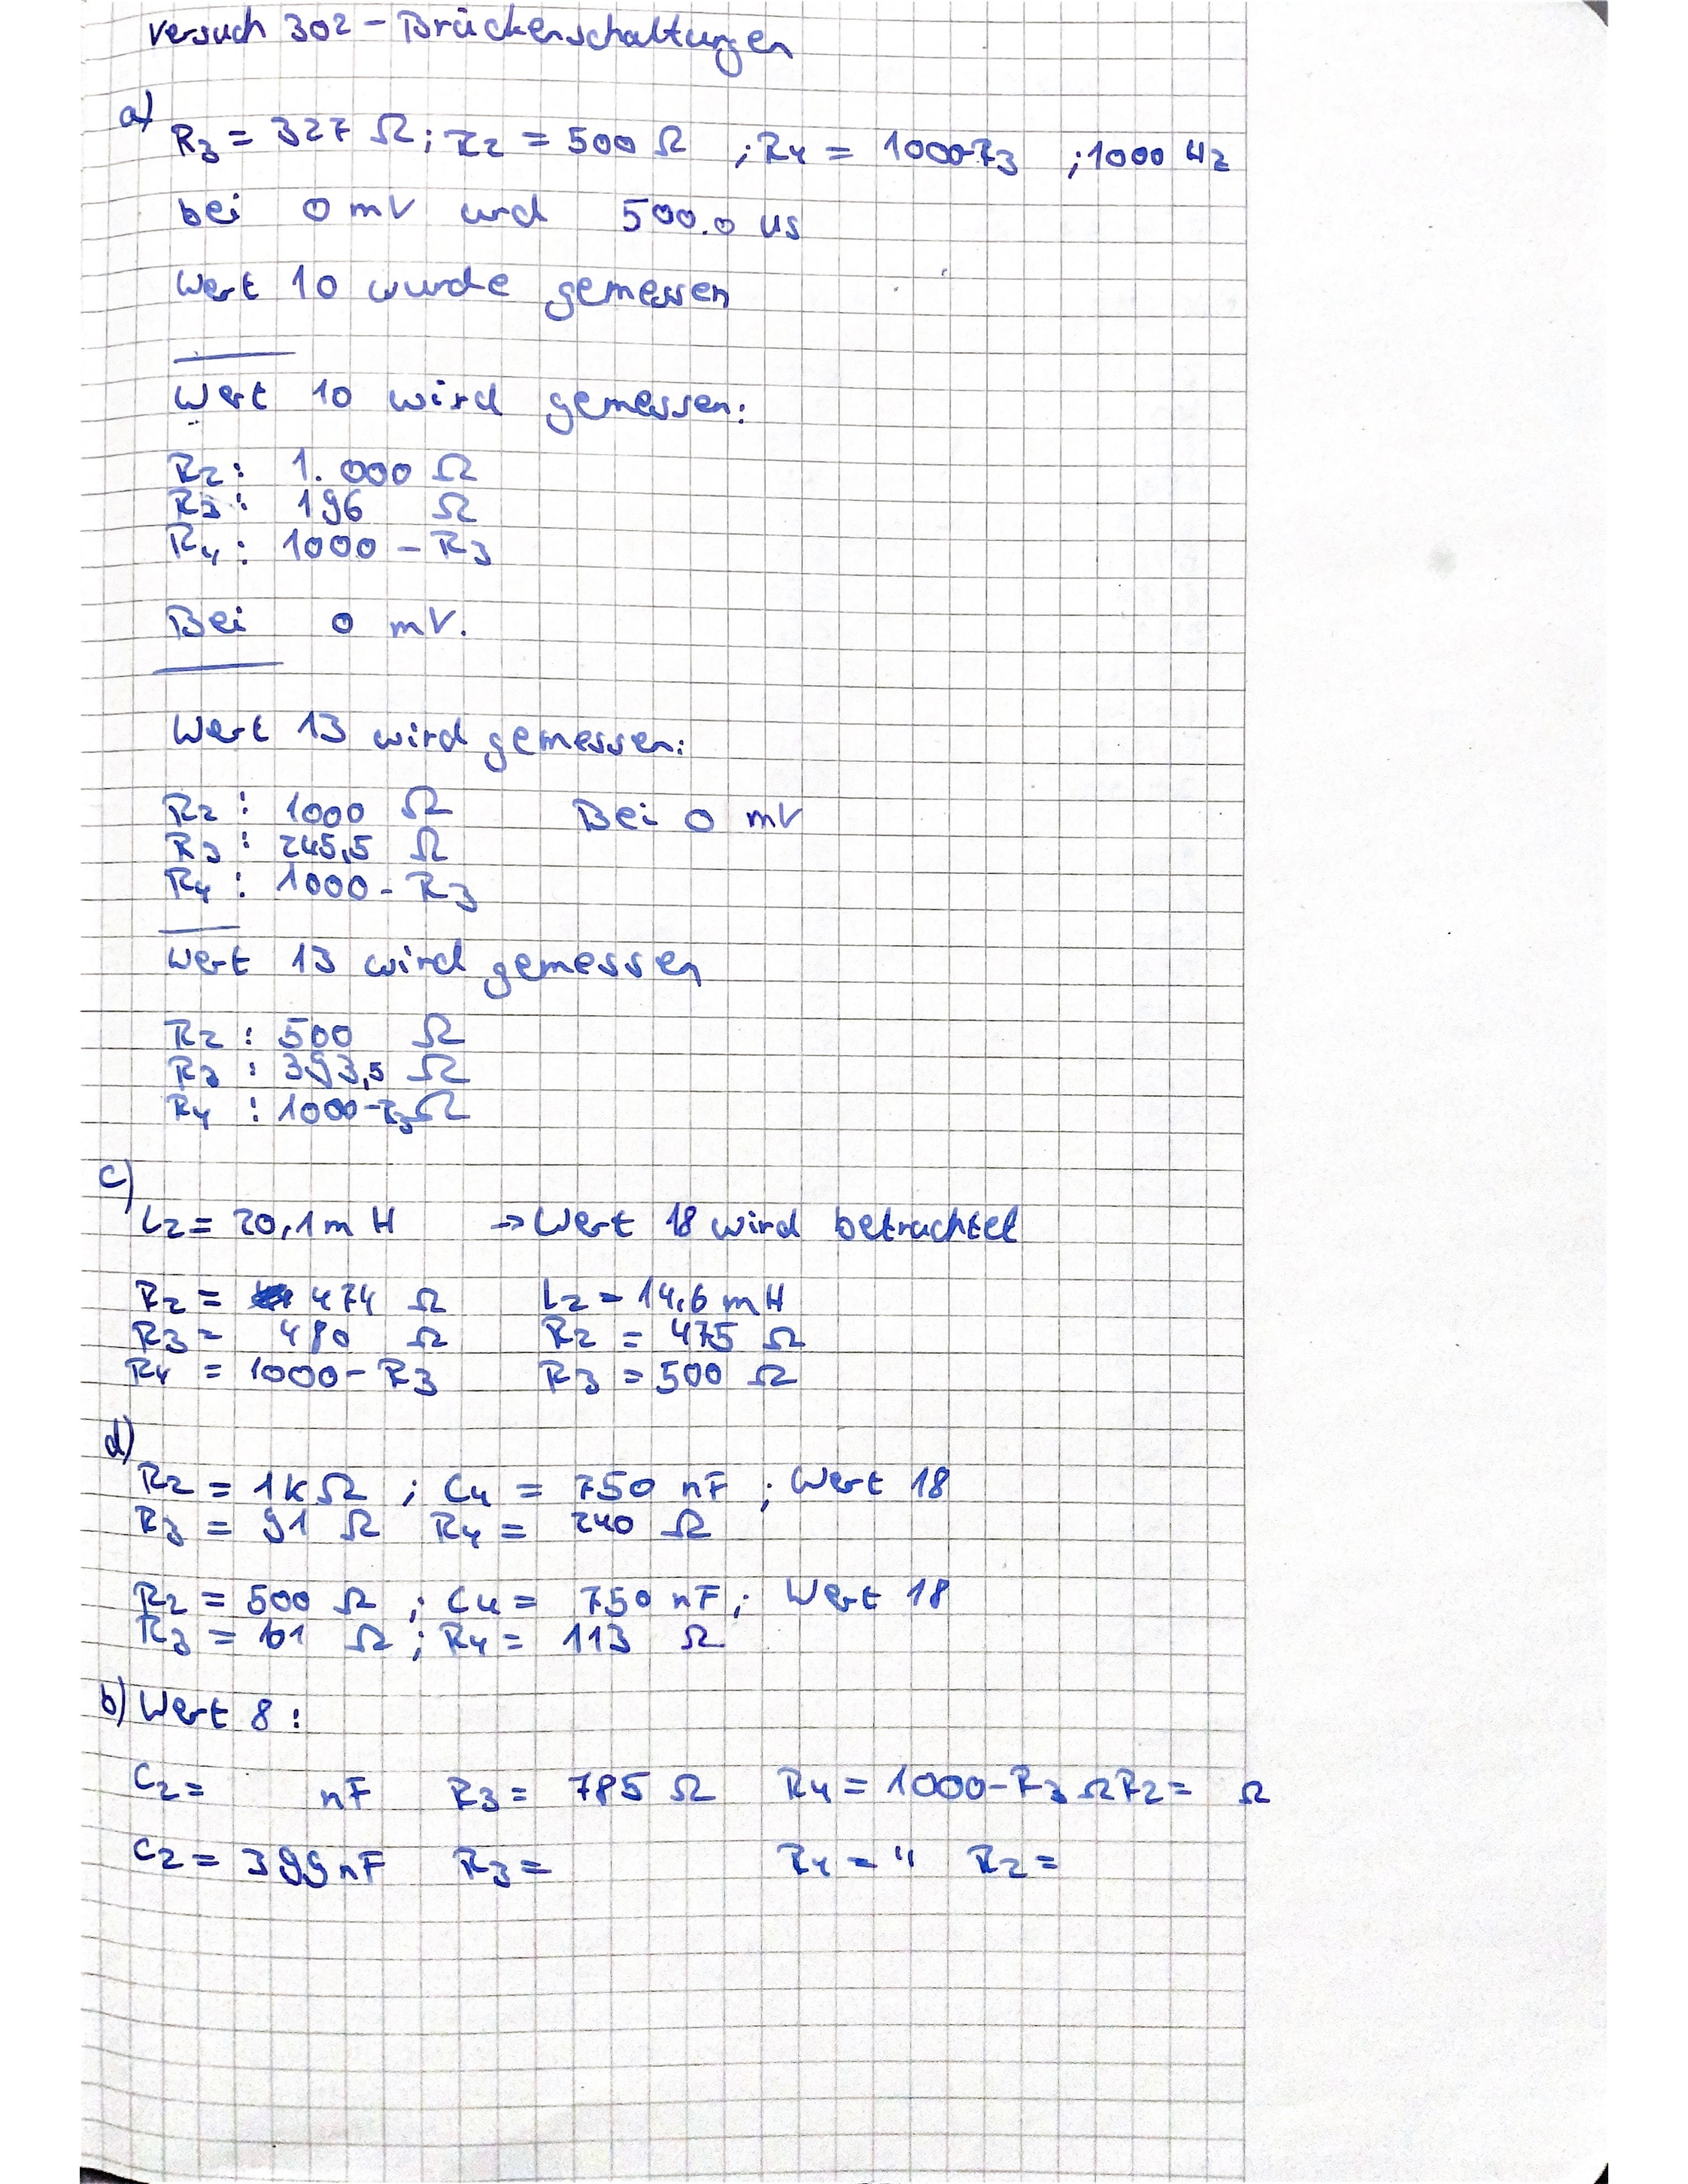
\includegraphics[width=0.75\textwidth]{dateien/daten1.jpg}
  \caption{Originale Messdaten.}
  \label{fig:daten1}
\end{figure}

\begin{figure}
  \centering
  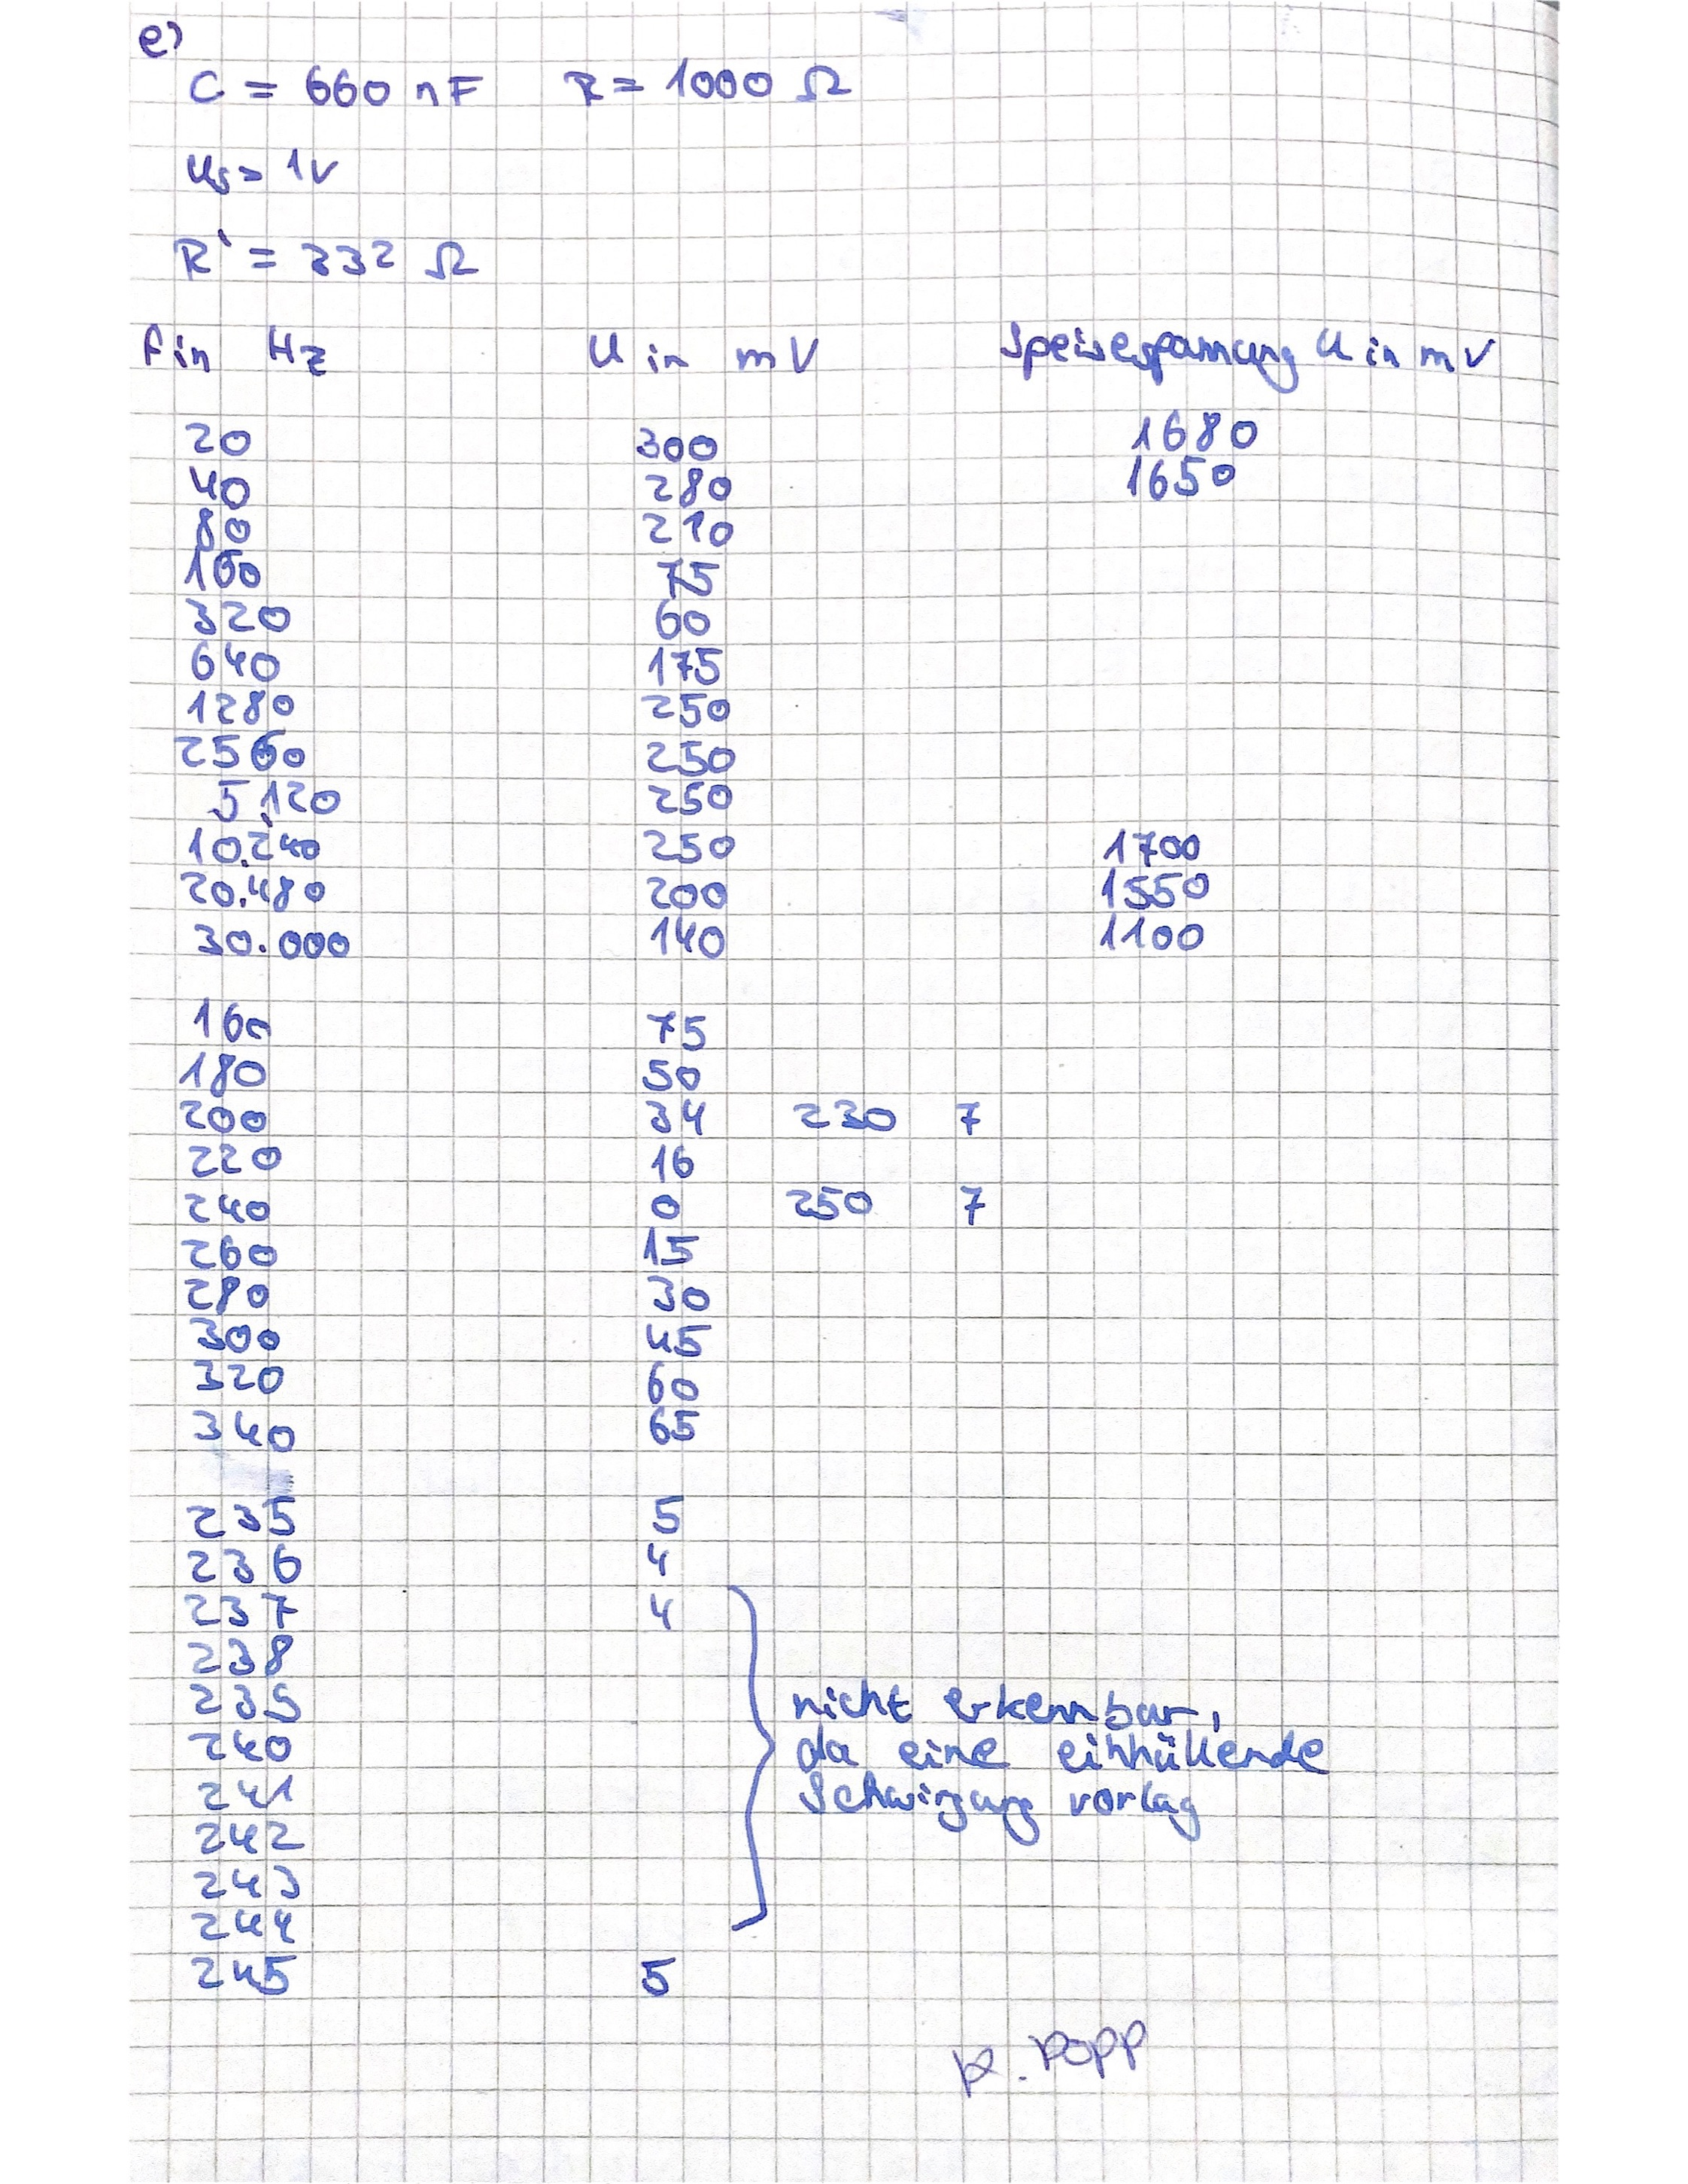
\includegraphics[width=0.75\textwidth]{dateien/daten2.jpg}
  \caption{Originale Messdaten.}
  \label{fig:daten2}
\end{figure}